%%%%%%%%%%%%%%%%%%%%%%%%%%%%%%%%%%%%%%%%%
% Short Sectioned Assignment
% LaTeX Template
% Version 1.0 (5/5/12)
%
% This template has been downloaded from:
% http://www.LaTeXTemplates.com
%
% Original author:
% Frits Wenneker (http://www.howtotex.com)
%
% License:
% CC BY-NC-SA 3.0 (http://creativecommons.org/licenses/by-nc-sa/3.0/)
%
%%%%%%%%%%%%%%%%%%%%%%%%%%%%%%%%%%%%%%%%%

%----------------------------------------------------------------------------------------
%	PACKAGES AND OTHER DOCUMENT CONFIGURATIONS
%----------------------------------------------------------------------------------------

\documentclass[paper=a4, fontsize=11pt]{scrartcl} % A4 paper and 11pt font size

\usepackage[T1]{fontenc} % Use 8-bit encoding that has 256 glyphs
\usepackage{fourier} % Use the Adobe Utopia font for the document - comment this line to return to the LaTeX default
\usepackage{amsmath,amsfonts,amsthm} % Math packages
\usepackage{natbib}
\usepackage{pgfplots}

\usepackage[utf8]{inputenc} 
\usepackage[ngerman]{babel}

\usepackage{latexsym}
\usepackage{textcomp}
\usepackage[T1]{fontenc}
\usepackage{bm}% bold math
\usepackage{hyperref}
\usepackage{graphicx}
\usepackage{caption}
\usepackage{sidecap}
\usepackage{subcaption}
\usepackage{verbatim}
\usepackage{epsfig}
\usepackage{framed,color}
\usepackage[usenames,dvipsnames]{pstricks}
\usepackage{epsfig}
\usepackage{tikz}
\usepackage{lipsum} % Used for inserting dummy 'Lorem ipsum' text into the template
\usepackage{sectsty} % Allows customizing section commands
\allsectionsfont{\centering \normalfont\scshape} % Make all sections centered, the default font and small caps
\usepackage{fancyhdr} % Custom headers and footers
\pagestyle{plain} % Makes all pages in the document conform to the custom headers and footers
\fancyhead{} % No page header - if you want one, create it in the same way as the footers below
\fancyfoot[L]{} % Empty left footer
\fancyfoot[C]{} % Empty center footer
\fancyfoot[R]{\thepage} % Page numbering for right footer
%\renewcommand{\headrulewidth}{0pt} % Remove header underlines
%\renewcommand{\footrulewidth}{0pt} % Remove footer underlines
\setlength{\headheight}{13.6pt} % Customize the height of the header
\usepackage{eso-pic}
\numberwithin{equation}{section} % Number equations within sections (i.e. 1.1, 1.2, 2.1, 2.2 instead of 1, 2, 3, 4)
\numberwithin{figure}{section} % Number figures within sections (i.e. 1.1, 1.2, 2.1, 2.2 instead of 1, 2, 3, 4)
\numberwithin{table}{section} % Number tables within sections (i.e. 1.1, 1.2, 2.1, 2.2 instead of 1, 2, 3, 4)

\setlength\parindent{0pt} % Removes all indentation from paragraphs - comment this line for an assignment with lots of text

%----------------------------------------------------------------------------------------
%	TITLE SECTION
%----------------------------------------------------------------------------------------

\newcommand{\horrule}[1]{\rule{\linewidth}{#1}} % Create horizontal rule command with 1 argument of height

\title{ 
\normalfont \normalsize 
\textsc{Albert-Ludwigs-Universität Freiburg} \\ [25pt] % Your university, school and/or department name(s)
\horrule{0.5pt} \\[0.4cm] % Thin top horizontal rule
\huge Rastertunnelmikroskop \\ % The assignment title
\horrule{2pt} \\[0.5cm] % Thick bottom horizontal rule
}

\author{Friedrich Schüßler und Volker Karle} % Your name

\date{\normalsize\today} % Today's date or a custom date

\begin{document}
\maketitle

\tableofcontents
\thispagestyle{empty}
\newpage
\setcounter{page}{1}


%----------------------------------------------------------------------------------------
%	PROBLEM 1
%----------------------------------------------------------------------------------------

%\part{Versuchsprotokoll}
\section{Durchführung des Versuchs}

Die Durchführung des Versuches gestaltete sich deutlich schwieriger als zuvor angenommen. 
Erst im Laufe des zweiten Versuchstages gelang uns eine Aufnahme der Graphitoberfläche mit 
atomarer Auflösung. Als Ursache ist vor allem die Verwendung unbrauchbarer Spitzen zu sehen, 
deren Unbrauchbarkeit jedoch erst nach langer Zeit bemerkbar wurde. Dazu kamen immer wieder 
kleinere Probleme mit dem Messgerät, bei dem zum Teil wichtige Funktionen versagten. Aus 
zeitlichen Gründen konnte nur Graphit und Gold untersucht werden.  

\subsection{Ablauf des Experiments nach Laborprotokoll}
Die gesamten Untersuchunge wurden im 'constant current'-Betriebsmodus gemacht. Dabei wurde 
der Strom in fast allen Fällen bei der Standarteinstellung $I = 1\mathrm{nA}$ belassen. 
Ausnahmen davon sind extra markiert worden. 
Die ersten Versuche wurden, soweit nicht anders angegeben,  mit den Standarteinstellungen 
des Programms unternommen. Zu den ersten Versuchen mit gebrauchten Spitzen zum Kennenlernen 
des Programms gibt es keine Aufzeichnungen.
Die Herstellung der Spitze hat einiges an Übung erfordert. Bei den ersten Spitzen hat das 
Reißen nicht geklappt, sodass ein unter der Lupe relativ glatter Schnitt zu erkennen war. 
Brauchbare Ergebnisse lieferten diese Spitzen nicht. Die meisten Spitzen, die wir verwendeten, 
waren aus alten Spitzen 'recycelt', indem an der Spitze nachgeschnitten bzw. neu abgerissen 
wurde. Tendenziell bessere Ergebnisse lieferten die Spitzen die direkt vom langen Draht 
abgerissen wurden, da hier das Abreißen einfacher zu realisieren war. In der folgenden Tabelle 
sind 'recycelte' Spitzen mit 'r', ohne Weiterbehandlung wiederverwendete mit 
'w' und neue Spitzen mit 'n' gekennzeichnet. $U$ ist die Spannung, die an die Spitze angelegt 
wurde. Für die automatische Annäherung wurde jeweils mit ca. 80mV angefangen, danach bis 
in 10mV Schritten bis auf ca. 50mV gesenkt. Die Annäherungsgeschwindigkeit $v$ dabei leicht 
von 48\% bis 35\% heruntergefahren. 
\\\\
\newcommand{\EOL}{\\ \hline}
\begin{tabular}{|l | l | p{12cm}|}
\hline
$n$ & Spitze & Beschreibung \EOL
    1   & r & Spitze und Probe nach erfolgreicher Annäherung beim Abrastern 
kollidiert (bei 600nm Rasterlänge) \EOL
    2   & w & U bis minimal 50mV, auf verschiedenen Größenskalen kein Signal (I = 0) \EOL
    3   & r & U = 64mV, Symmetrische Struktur bei 600nm erkennbar, bei 180nm 
regelmäßige Struktur in der Größenordnung von 50nm zu erkennen, bei 10nm Rauschen 
(Abb. \ref{fig:graphit_01}) \EOL
    4   & r & unter der Lupe vielversprechendere Schnitt. 'Advance'-Funktion geht 
nicht. Ein Annähern mit der Hand führt zur Kollision \EOL
    5   & n & 'Advance'-Funktion nach Putzen sämtlicher Teile und Neustart des Systems wieder 
funktionstüchtig. Die ersten Messungen bei 600nm, 180nm und 30nm sind konsistent (es wurde 
jeweils auf den Bereich des Maximums vergrößert). Bei 10nm ist jedoch nur Rauschen zu erkennen.
(Abb. \ref{fig:graphit_02}). \EOL
    6   & r & Bei verschiedenen Spannungen nach vollendetem 'Approach' kein Signal \EOL
    7   & r & Gleiches Problem wie bei '6' \EOL
    8   & w & Kein gutes Signal, Spitze offenbar unbrauchbar
(Abb. \ref{fig:graphit_03}) \EOL
    9   & n & siehe weiter unten \EOL 
   10   & r & Kollision gemeldet nach Annäherung mit Geschwindigkeit 45\% bei
$U = 80\mathrm{mV}$, gemessener Tunnelstrom nicht homogen. \EOL
   11   & r & erneut Kollision bei erstem Scan und gleichen Einstellungen, bei kleineren 
Skalen (100nm, 10nm) lediglich Rauschen.  \EOL
\end{tabular}
\\\\
Anhand der neunten Spitze, die neu vom Draht gerissen wurde,  wird exemplarisch das Vorgehen 
dargestellt. Dabei ist $n$ der Schritt, $v$ die eingestellte Annäherungsgeschwindigkeit für 
die automatische Annäherung, $U$ die angelegte Spannung , $a$ die Skala 
und $z_{\mathrm{max}}$ der maximale berechnete Höhenunterschied.
\\\\
\begin{tabular}{|l |l |l |l |l |p{8cm}|}
\hline
$n$ & $v$ & $U$ & $a$ & $z_{\mathrm{max}}$ & Beobachtung \EOL
1   & 45\%  & 80mv  & 600nm & 27nm  & Symmetrische Struktur über den gesamten Scanbereich, 
starkes Rauschen 
(Abb. \ref{fig:graphit_04_01}) \EOL
2   & 40\%  & 60mv  & 100nm & 2.7nm  & Fast ausschließlich Rauschen zu erkennen, leichte 
Wölbung, Tunnelstrom $I$ nicht konstant 
(Abb. \ref{fig:graphit_04_02}) \EOL
3   & 38\%  & 50mv  & 10nm & 1.4nm  & Horizontale Linien (Rauschen) bei konstantem $I$, 
keine Gitterstruktur erkennbar.
(Abb. \ref{fig:graphit_04_03}) \EOL
\end{tabular}
\\\\
Der erste und einzige erfolgreiche Versuch wurde mit der 12. Spitze, die wiederum neu 
abgerissen wurde, unternommen. In der folgenden Tabelle sind die einzelnen Schritte 
aufgelistet. Die automatische Annährungsgeschwindigkeit liegt mit Ausnahme des ersten 
Schrittes (46\%) immer bei 40\%, der Tunnelstrom $I$ bei 1nA (mit Ausnahme des letzten 
Schrittes mit 2nA). Mit 'px/l' ist die Anzahl der Messpunkte bzw. Pixel pro Linie und 
damit auch die Anzahl der Linien in z-Richtung bezeichnet, mit $t$ die Zeit, die pro 
Abfahren einer Linie. 
\\\\
\begin{tabular}{|p{5pt} |p{18pt} |p{12pt} |p{14pt} |p{12pt} |p{12pt} |p{16pt} |p{10cm}|}
\hline
$n$ & Abb.      & $\frac{U}{\mathrm{mV}}$ & $\frac{\mathrm{px}}{\mathrm{l}}$ & 
    $\frac{t}{\mathrm{s}}$ & $\frac{a}{\mathrm{nm}} $ & 
    $\frac{z_{\mathrm{max}}}{\mathrm{nm}}$ & Beobachtung \EOL
1   & \ref{fig:graphit_06_01}& 80 & 128 & 0.4 & 600 & 17 & großflächige Struktur mit 
Stufen und konstanter Höhe im Zentrum; Wiederholung der Messung bei 55mV ergab keine 
sichtbare Veränderung \EOL
2   & \ref{fig:graphit_06_02}& 55 & 256 & 0.4 & 180 & 2.36 & Vergrößerung in den Bereich bei 
ca. $(x, y) = (500\mathrm{nm}, 0\mathrm{nm})$ im Bezug auf Abb \ref{fig:graphit_06_01}; 
Abstufungen und Interferenzartige Ringe zu erkennen \EOL
3   & \ref{fig:graphit_06_03}& 55 & 256 & 0.4 &  30 & 0.27 & Trotz Rauschen ist eine 
regelmäßige Struktur zu erkennen \EOL
4   & \ref{fig:graphit_06_04}& 55 & 256 & 0.4 &  10 & 0.16 & Gitter aus gerade angeordneten 
Punkten sichtbar\EOL
5   & \ref{fig:graphit_06_05}& 55 & 256 & 0.4 &  10 & 0.21 & Wiederholung an gleicher Stelle, 
verzogenes Bild mit schlechterer Auflösung. Wärmedrift?\EOL
6   & \ref{fig:graphit_06_06}& 55 & 128 & 0.4 &   3 & 0.16 & \EOL
7   & \ref{fig:graphit_06_07}& 55 & 256 & 0.8 &   3 & 0.16 & Wiederholung an gleicher Stelle, 
starkes Rauschen, stark verzogen: Wärmedrift, zu langsam?\EOL
8   & \ref{fig:graphit_06_08}& 45 & 256 & 0.8 &   3 & 0.16 & trotz starken Rauschens Punkte 
sichtbar \EOL
9  & \ref{fig:graphit_06_09}& 35 & 256 & 0.8 &   3 & 0.27 & Rauschen und Drift erkennbar, 
keine Punkte mehr zu sehen \EOL 
10  & \ref{fig:graphit_06_10}& 35 & 256 & 0.8 &  30 & 1.55 & Wechsel der Position, jetzt bei 
ca. $(x, y) = (100\mathrm{nm}, 450\mathrm{nm})$ im Bezug auf Abb \ref{fig:graphit_06_01}; Stufe zu erkennen, 
starkes Rauschen \EOL
11  & \ref{fig:graphit_06_11}& 35 & 256 & 0.8 &  10 & 0.27 & Streifen mit unterschiedlich 
guter Auflösung, Gitter im unteren Streifen gut zu erkennen \EOL
12  & \ref{fig:graphit_06_12}& 35 & 256 & 0.8 &  10 & 0.27 & Abschirmbox zum ersten Mal benutzt 
(während des Messvorgangs - Störung als schwarzer Streifen bei $y \approx 1\mathrm{nm}$ 
erkennbar); das vorher sehr verrauschte Bild ist etwas besser; weiterhin Bänder mit 
unterschiedlicher Auflösung und Drift \EOL
13  & \ref{fig:graphit_06_13}& 35 & 256 & 0.8 &   3 & 0.27 & Rauschen, kaum Struktur zu 
erkennen\EOL 
14  & \ref{fig:graphit_06_14}& 35 & 256 & 0.8 &   3 & 0.21 & Wiederholung der Messung 14, 
deutlich besseres Bild; auf parallel angeordneten Streifen liegende, punktförmige 
Erhöhungen, die annähernd gleichseitige Dreiecke bilden, wie es für die Abbildung der 
Oberfläche von Graphit erwartet wurde. \EOL 
15  & \ref{fig:graphit_06_15}& 35 & 256 & 0.8 & 0.8 & 0.16 & fast ausschließlich Rauschen zu 
erkennen \EOL
16  & \ref{fig:graphit_06_16}& 35 & 256 & 0.8 & 1.6 & 0.16 & regelmäßig angeordnete Punkte 
wegen starken Rauschens nur andeutungsweise zu erkennen \EOL
17  & \ref{fig:graphit_06_17}& 35 & 256 & 0.8 & 3.2 & 0.27 & nach Veränderung des Regelstromes 
deutlich schlechtere Bildqualität als bei Versuch 15; Streifen mit starker Störung \EOL
\end{tabular}

%%%%%%%%%%%%%%%%%%%%%%%%%%%%%%%%%%%%%%%%%%%%%%%%%%%%%%%%%
%       Messung Gold
%%%%%%%%%%%%%%%%%%%%%%%%%%%%%%%%%%%%%%%%%%%%%%%%%%%%%%%%%
Die Oberfläche von Gold haben wir mit zwei Spitzen vermessen. In beiden Fällen waren entweder die 
Parameter nicht optimal eingestellt oder die Spitzen nicht geeignet, um die atomare Oberflächenstruktur 
aufzulösen. Es konnte mit der zweiten Spitze interessante Strukturen auf einer Skala von ca. 200nm aufgelöst 
werden. Es folgt ein tabellarischer Überblick des Versuchsablaufs. Die Mehrzahl der Bilder vollkommen 
verrauschter Aufnahmen wurde nciht mit in den Anhang aufgenommen. 
\\\\
\begin{tabular}{|p{5pt} |p{18pt} |p{12pt} |p{14pt} |p{12pt} |p{12pt} |p{16pt} |p{10cm}|}
\hline
$n$ & Abb.      & $\frac{U}{\mathrm{mV}}$ & $\frac{\mathrm{px}}{\mathrm{l}}$ & 
    $\frac{t}{\mathrm{s}}$ & $\frac{a}{\mathrm{nm}} $ & 
    $\frac{z_{\mathrm{max}}}{\mathrm{nm}}$ & Beobachtung \EOL
1   & \ref{fig:gold_01_01}& 70 & 128 & 0.8 &   3 &13.8 & Rauschen, sehr große Höhenunterschiede 
angegeben \EOL
2   &                     & 70 & 128 & 0.8 & 100 & 140 & Kollision, 140nm Höhendifferenz angegeben. \EOL
3   & \ref{fig:gold_01_03}& 70 & 128 & 0.8 &  30 & 8.6 & Stark verrauscht. Geometrische Strukturen 
nicht zu interpretieren. \EOL
4   & \ref{fig:gold_01_04}& 40 & 128 & 0.4 &   7 & 1.2 & Rauschen\EOL
5   & \ref{fig:gold_01_05}& 40 & 256 & 0.4 &   7 & 0.8 & Rauschen\EOL
\end{tabular}
\\\\

\begin{tabular}{|p{5pt} |p{18pt} |p{12pt} |p{14pt} |p{12pt} |p{12pt} |p{16pt} |p{10cm}|}
\hline
$n$ & Abb.      & $\frac{U}{\mathrm{mV}}$ & $\frac{\mathrm{px}}{\mathrm{l}}$ & 
    $\frac{t}{\mathrm{s}}$ & $\frac{a}{\mathrm{nm}} $ & 
    $\frac{z_{\mathrm{max}}}{\mathrm{nm}}$ & Beobachtung \EOL
1   & \ref{fig:gold_02_01}& 60 & 128 & 0.8 & 600 & 2.3 & Großflächige, sehr flache Strukturen\EOL
2   & \ref{fig:gold_02_02}& 60 & 128 & 0.8 & 180 & 0.8 & Leicht verrauscht, trotzdem sind facettenartige 
Strukturen zu erkennen. \EOL
3   & \ref{fig:gold_02_03}& 60 & 128 & 0.8 &  30 & 0.3 & Rauschen \EOL 
4   & & 45 & 256 & 0.8 &  30 & 0.3 & Rauschen \EOL 
5   & & 45 & 256 & 0.8 &   8 & 0.3 & Rauschen \EOL 
6   & & 45 & 256 & 0.4 &   3 & 0.5 & Rauschen \EOL
7   & & 35 & 256 & 0.4 &  20 & 0.5 & Rauschen \EOL 
8   & & 35 & 256 & 0.4 &  30 & 1.0 & Rauschen \EOL
\end{tabular}



%%%%%%%%%%%%%%%%%%%%%%%%%%%%%%%%%%%%%%%%%%%%%%%%%%%%%%%%%
%       Bilder Graphit
%%%%%%%%%%%%%%%%%%%%%%%%%%%%%%%%%%%%%%%%%%%%%%%%%%%%%%%%%
\newcommand{\picwidth}{0.45\textwidth}
\centering
\begin{figure}
    \begin{subfigure}[b]{\picwidth}
        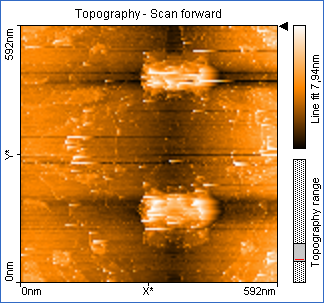
\includegraphics[width=\textwidth]{data/Graphit/pic_01_01_600nm}
        \caption{}
        \label{fig:graphit_01_01}
    \end{subfigure}\qquad
    \begin{subfigure}[b]{\picwidth}
        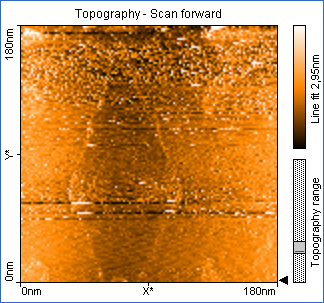
\includegraphics[width=\textwidth]{data/Graphit/pic_01_02_180nm}
        \caption{}
        \label{fig:graphit_01_02}
    \end{subfigure}
    \begin{subfigure}[b]{\picwidth}
        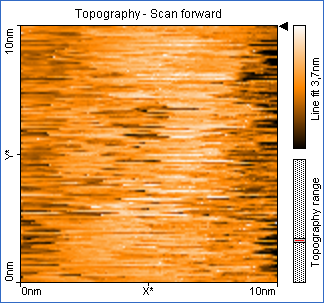
\includegraphics[width=\textwidth]{data/Graphit/pic_01_03_10nm}
        \caption{}
        \label{fig:graphit_01_03}
    \end{subfigure}
    \caption{STM-Aufnahmen von Graphit, Spitze Nr. 3}\label{fig:graphit_01}
\end{figure}

\begin{figure}
    \begin{subfigure}[b]{\picwidth}
        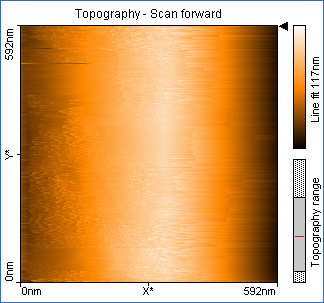
\includegraphics[width=\textwidth]{data/Graphit/pic_02_01_600nm}
        \caption{}
        \label{fig:graphit_02_01}
    \end{subfigure}\qquad
    \begin{subfigure}[b]{\picwidth}
        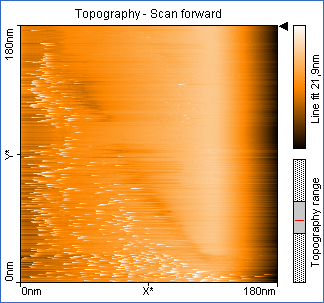
\includegraphics[width=\textwidth]{data/Graphit/pic_02_02_180nm}
        \caption{}
        \label{fig:graphit_02_02}
    \end{subfigure}
    \begin{subfigure}[b]{\picwidth}
        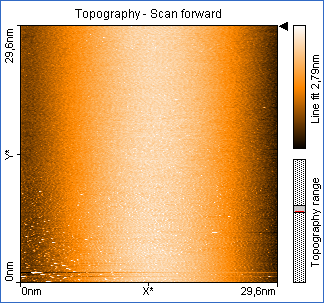
\includegraphics[width=\textwidth]{data/Graphit/pic_02_03_30nm}
        \caption{}
        \label{fig:graphit_02_03}
    \end{subfigure}\qquad
    \begin{subfigure}[b]{\picwidth}
        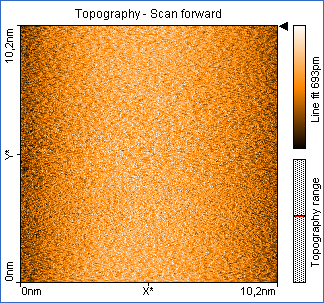
\includegraphics[width=\textwidth]{data/Graphit/pic_02_04_10nm}
        \caption{}
        \label{fig:graphit_02_04}
    \end{subfigure}
    \caption{STM-Aufnahmen von Graphit, Spitze Nr. 5}\label{fig:graphit_02}
\end{figure}

\begin{figure}
    \begin{subfigure}[b]{\picwidth}
        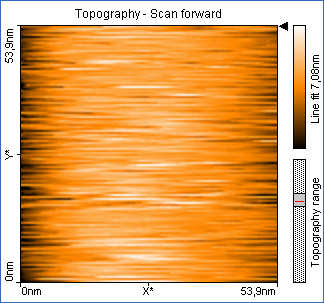
\includegraphics[width=\textwidth]{data/Graphit/pic_03_01_50nm}
        \caption{}
        \label{fig:graphit_03_01}
    \end{subfigure}\qquad
    \begin{subfigure}[b]{\picwidth}
        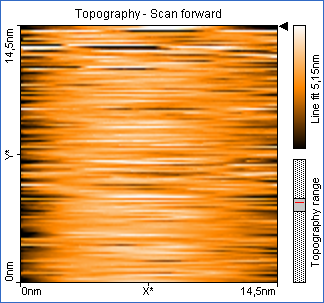
\includegraphics[width=\textwidth]{data/Graphit/pic_03_02_15nm}
        \caption{}
        \label{fig:graphit_03_02}
    \end{subfigure}
    \caption{STM-Aufnahmen von Graphit, Spitze Nr. 8}\label{fig:graphit_03}
\end{figure}

\begin{figure}
    \begin{subfigure}[b]{\picwidth}
        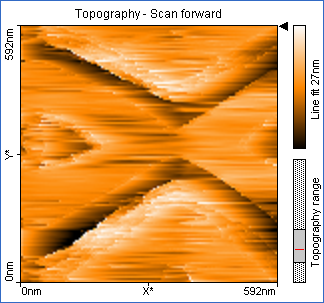
\includegraphics[width=\textwidth]{data/Graphit/pic_04_01_600nm}
        \caption{}
        \label{fig:graphit_04_01}
    \end{subfigure}\qquad
    \begin{subfigure}[b]{\picwidth}
        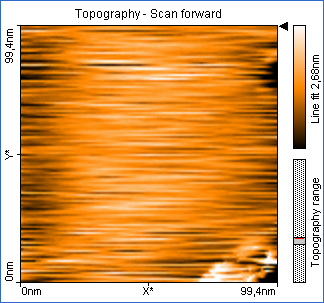
\includegraphics[width=\textwidth]{data/Graphit/pic_04_02_100nm}
        \caption{}
        \label{fig:graphit_04_02}
    \end{subfigure}
    \begin{subfigure}[b]{\picwidth}
        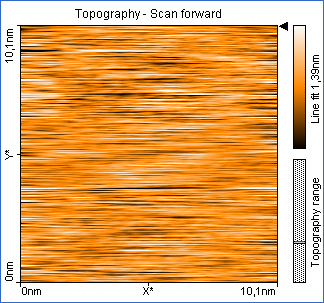
\includegraphics[width=\textwidth]{data/Graphit/pic_04_03_10nm}
        \caption{}
        \label{fig:graphit_04_03}
    \end{subfigure}
    \caption{STM-Aufnahmen von Graphit, Spitze Nr. 9}\label{fig:graphit_04}
\end{figure}

\begin{figure}
    \begin{subfigure}[b]{\picwidth}
        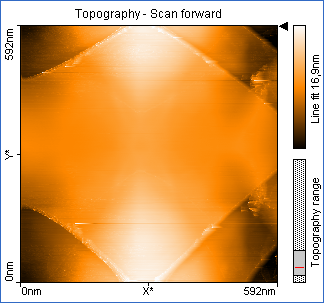
\includegraphics[width=\textwidth]{data/Graphit/pic_06_01_600nm}
        \caption{}
        \label{fig:graphit_06_01}
    \end{subfigure}\qquad
    \begin{subfigure}[b]{\picwidth}
        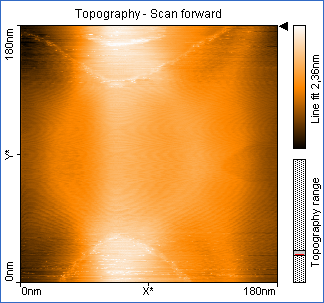
\includegraphics[width=\textwidth]{data/Graphit/pic_06_02_180nm}
        \caption{}
        \label{fig:graphit_06_02}
    \end{subfigure}
    \begin{subfigure}[b]{\picwidth}
        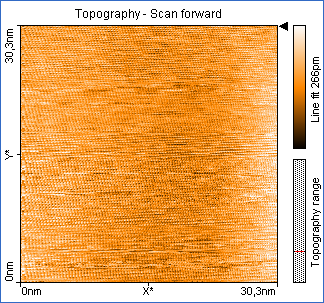
\includegraphics[width=\textwidth]{data/Graphit/pic_06_03_30nm}
        \caption{}
        \label{fig:graphit_06_03}
    \end{subfigure}\qquad
    \begin{subfigure}[b]{\picwidth}
        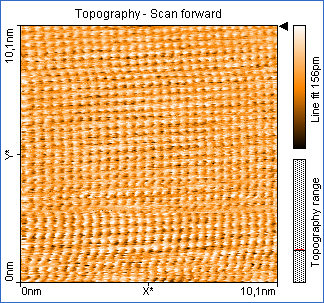
\includegraphics[width=\textwidth]{data/Graphit/pic_06_04_10nm}
        \caption{}
        \label{fig:graphit_06_04}
    \end{subfigure}
    \begin{subfigure}[b]{\picwidth}
        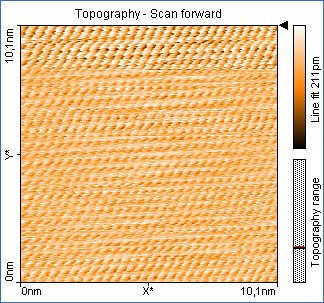
\includegraphics[width=\textwidth]{data/Graphit/pic_06_05_10nm}
        \caption{}
        \label{fig:graphit_06_05}
    \end{subfigure}\qquad
    \begin{subfigure}[b]{\picwidth}
        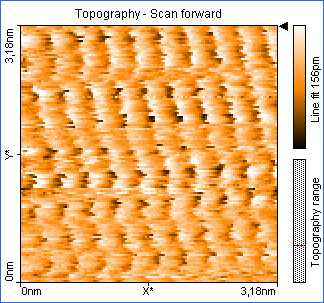
\includegraphics[width=\textwidth]{data/Graphit/pic_06_06_3nm}
        \caption{}
        \label{fig:graphit_06_06}
    \end{subfigure}
    \caption{STM-Aufnahmen von Graphit, Spitze Nr. 12, Messungen 1 bis 6}\label{fig:graphit_06}
\end{figure}

\begin{figure}
    \begin{subfigure}[b]{\picwidth}
        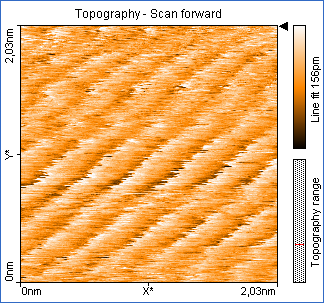
\includegraphics[width=\textwidth]{data/Graphit/pic_06_07_3nm}
        \caption{}
        \label{fig:graphit_06_07}
    \end{subfigure}\qquad
    \begin{subfigure}[b]{\picwidth}
        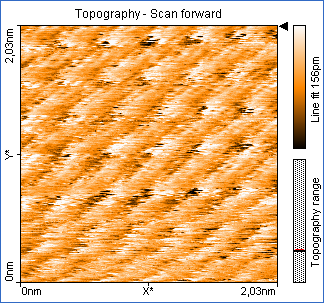
\includegraphics[width=\textwidth]{data/Graphit/pic_06_08_3nm}
        \caption{}
        \label{fig:graphit_06_08}
    \end{subfigure}
    \begin{subfigure}[b]{\picwidth}
        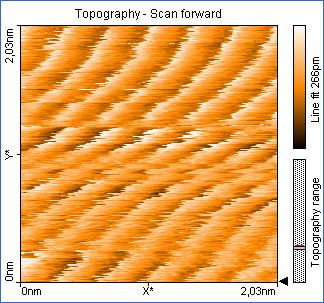
\includegraphics[width=\textwidth]{data/Graphit/pic_06_09_3nm}
        \caption{}
        \label{fig:graphit_06_09}
    \end{subfigure}\qquad
    \begin{subfigure}[b]{\picwidth}
        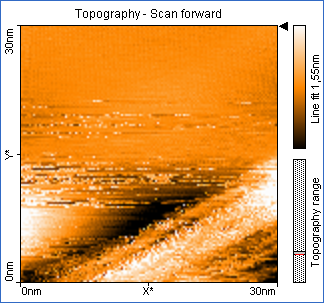
\includegraphics[width=\textwidth]{data/Graphit/pic_06_10_30nm}
        \caption{}
        \label{fig:graphit_06_10}
    \end{subfigure}
    \begin{subfigure}[b]{\picwidth}
        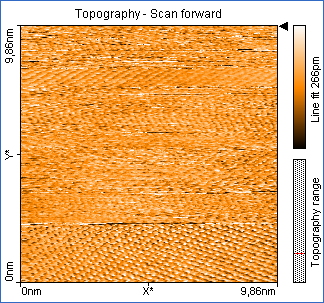
\includegraphics[width=\textwidth]{data/Graphit/pic_06_11_10nm}
        \caption{}
        \label{fig:graphit_06_11}
    \end{subfigure}\qquad
    \begin{subfigure}[b]{\picwidth}
        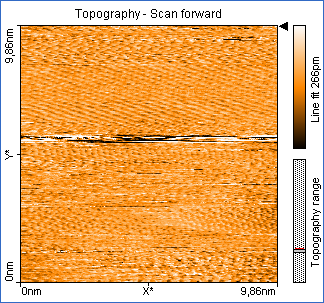
\includegraphics[width=\textwidth]{data/Graphit/pic_06_12_10nm}
        \caption{}
        \label{fig:graphit_06_12}
    \end{subfigure}
    \caption{STM-Aufnahmen von Graphit, Spitze Nr. 12, Messungen 7 - 12}\label{fig:graphit_06}
\end{figure}

\begin{figure}
    \begin{subfigure}[b]{\picwidth}
        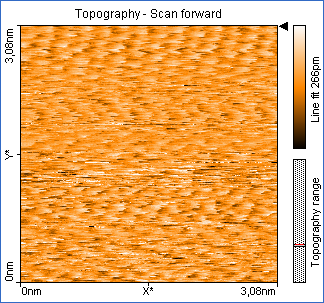
\includegraphics[width=\textwidth]{data/Graphit/pic_06_13_3nm}
        \caption{}
        \label{fig:graphit_06_13}
    \end{subfigure}\qquad
    \begin{subfigure}[b]{\picwidth}
        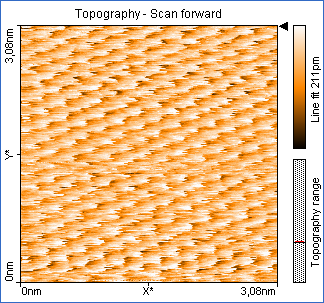
\includegraphics[width=\textwidth]{data/Graphit/pic_06_14_3nm}
        \caption{}
        \label{fig:graphit_06_14}
    \end{subfigure}
    \begin{subfigure}[b]{\picwidth}
        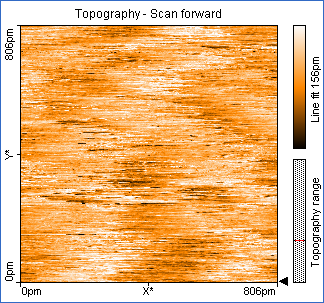
\includegraphics[width=\textwidth]{data/Graphit/pic_06_15_800pm}
        \caption{}
        \label{fig:graphit_06_15}
    \end{subfigure}\qquad
    \begin{subfigure}[b]{\picwidth}
        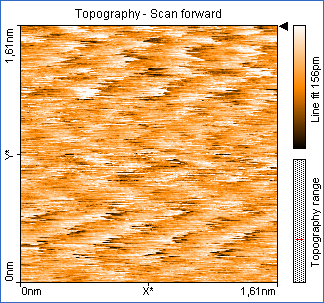
\includegraphics[width=\textwidth]{data/Graphit/pic_06_16_1600pm}
        \caption{}
        \label{fig:graphit_06_16}
    \end{subfigure}
    \begin{subfigure}[b]{\picwidth}
        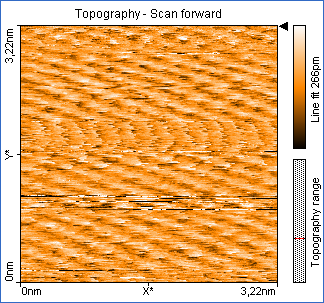
\includegraphics[width=\textwidth]{data/Graphit/pic_06_17_3nm_set_point_2nA}
        \caption{}
        \label{fig:graphit_06_17}
    \end{subfigure}
    \caption{STM-Aufnahmen von Graphit, Spitze Nr. 12, Messungen 13 - 17}\label{fig:graphit_06}
\end{figure}

%%%%%%%%%%%%%%%%%%%%%%%%%%%%%%%%%%%%%%%%%%%%%%%%%%%%%%%%%
%       Bilder Gold
%%%%%%%%%%%%%%%%%%%%%%%%%%%%%%%%%%%%%%%%%%%%%%%%%%%%%%%%%

\begin{figure}
    \begin{subfigure}[b]{\picwidth}
        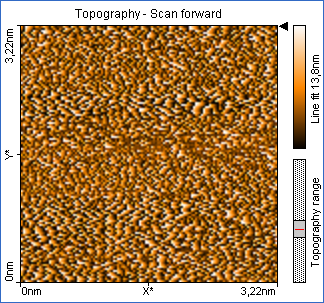
\includegraphics[width=\textwidth]{data/Gold/pic_01_01_3nm}
        \caption{}
        \label{fig:gold_01_01}
    \end{subfigure}\qquad
    \begin{subfigure}[b]{\picwidth}
        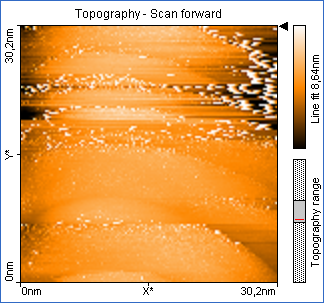
\includegraphics[width=\textwidth]{data/Gold/pic_01_03_30nm}
        \caption{}
        \label{fig:gold_01_03}
    \end{subfigure}
    \begin{subfigure}[b]{\picwidth}
        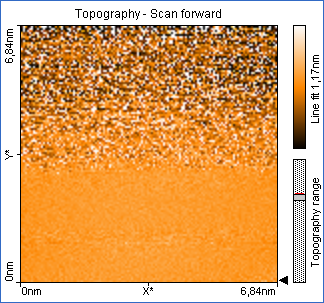
\includegraphics[width=\textwidth]{data/Gold/pic_01_04_6nm}
        \caption{}
        \label{fig:gold_01_04}
    \end{subfigure}\qquad
    \begin{subfigure}[b]{\picwidth}
        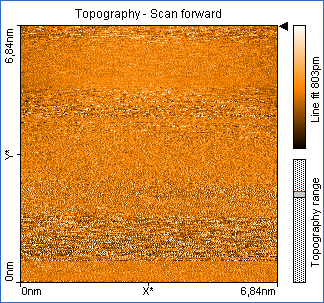
\includegraphics[width=\textwidth]{data/Gold/pic_01_05_6nm}
        \caption{}
        \label{fig:gold_01_05}
    \end{subfigure}
    \caption{STM-Aufnahmen von Gold, Spitze Nr. 1}\label{fig:gold_02}
\end{figure}

\begin{figure}
    \begin{subfigure}[b]{\picwidth}
        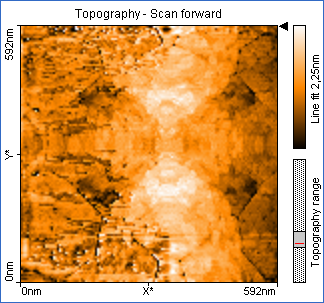
\includegraphics[width=\textwidth]{data/Gold/pic_02_01_600nm}
        \caption{}
        \label{fig:gold_02_01}
    \end{subfigure}\qquad
    \begin{subfigure}[b]{\picwidth}
        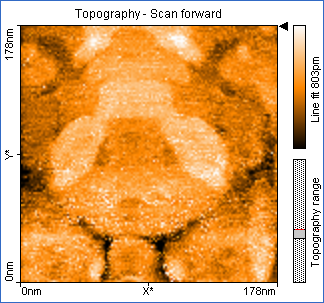
\includegraphics[width=\textwidth]{data/Gold/pic_02_02_180nm}
        \caption{}
        \label{fig:gold_02_02}
    \end{subfigure}
    \begin{subfigure}[b]{\picwidth}
        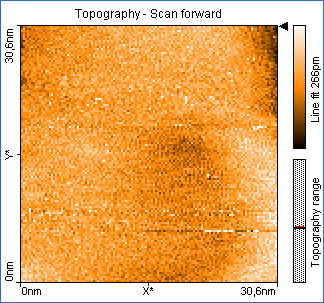
\includegraphics[width=\textwidth]{data/Gold/pic_02_03_30nm}
        \caption{}
        \label{fig:gold_02_03}
    \end{subfigure}
    \caption{STM-Aufnahmen von Gold, Spitze Nr. 2}\label{fig:gold_01}
\end{figure}
\flushleft




\bibliographystyle{plain}
\bibliography{Protokoll}
\end{document}
